% --------------------------------
  \chapter{Sobre el uso de \LaTeX}
% --------------------------------
\label{C:sobre_LaTeX}

\section{Introducción}

\LaTeX~ es un editor de texto bajo el paradigma de edición de texto ``lo que ve es lo que quiere decir'' (WYSIWYM, del inglés \emph{What You See Is What You Mean}) en el que se utiliza un lenguaje de descripción de formato\footnote{En ese sentido parecido al HTML}. Este paradigma es diferente a su contraparte y tradicional paradigma WYSIWYG (del inglés \emph{What You See Is What You Get}, ``lo que ve es lo que obtiene''), en el que se edita el texto y los demás elementos en una interfaz gráfica. Este es el caso de herramientas de ofimática como Microsoft Office, OpenOffice y LibreOffice y editores gráficos de todo tipo.

\begin{quote}
\LaTeX~ ``...es un sistema de composición lógica, por oposición a los sistemas de composición visual o programas WYSIWYG (\ldots) Con el sistema \LaTeX, lo que el autor escribe y ve en la pantalla del ordenador es el contenido del documento y su estructura lógica, pero entre estos y el documento compuesto hay un paso intermedio de procesamiento o \emph{compilación} del documento mediante el sistema \LaTeX'' \cite{Valiente2001}.
\end{quote}

Existe bibliografía extensa (incluyendo \cite{Valiente2001}\cite{Gratzer2001}\cite{Krishnan2003}\cite{Oetiker2014}\cite{Wikibooks2016}) donde se puede ampliar sobre \LaTeX. Así mismo, en Internet hay gran cantidad de tutoriales, comunidades y foros sobre el tema, como en \cite{StackExchange2016}. Se recomienda consultar estas fuentes para ampliar las posibilidades de escritura con este lenguaje.

En este capítulo se incluyen y explican algunos de los elementos básicos y más utilizados para la redacción en \LaTeX: ecuaciones, figuras, tablas, además de referencias a bibliografías, secciones, entre otras cosas, y puede ser utilizado como base para la elaboración del trabajo escrito del curso.

\subsection{¿Por qué \LaTeX? (opcional)}

\LaTeX~ es un paradigma de edición de texto utilizado ampliamente en la comunidad científica y tecnológica de todo el mundo, en publicaciones, revistas, libros y más. 

Tiene la virtud de facilitar la composición de un documento bien diseñado que ahorra toda la cuestión de forma para el editor.

La siguiente lista\footnote{Adaptado de \url{http://haptonstahl.org/latex/whyuse.php}} explica algunos puntos acerca del uso de \LaTeX.

\begin{description}

\item[Documentos estructurados] 
Es más fácil crear documentos estructurados en \LaTeX~ que en Word u otros editores. Un documento estructurado es un \emph{paper}, artículo, libro o tesis con capítulos, secciones, subsecciones, apéndices, tablas de contenidos, índices, etc. Los capítulos y secciones usualmente son enumerados secuencialmente, están listados en una tabla de contenidos, etc. Cuando se hacen cambios, todas las referencias relativas tienen que ser actualizadas. Todo esto es trivialmente fácil en \LaTeX.

Si no se quiere pensar acerca del formato y solo se quiere que el \emph{software} haga las cosas verse bien, hay que usar \LaTeX.

\item[Ecuaciones] 
Es más fácil y rápido escribir símbolos matemáticos utilizando \LaTeX~ que con MS Word. Una o dos páginas de fórmulas probablamente harán caer MS Word. Cientos de páginas de fórmulas no harán caer a \LaTeX.

\item[Calidad de tipografía e impresión] 
La escritura en \LaTeX~ es superior a la de otros procesadores de texto. Más referencias sobre esto en \url{http://nitens.org/taraborelli/latex}.

\end{description}

%%%%%%%%%%%%%%%%%%%%%%%%%%%%%%%%%%%%%%%%%%%%%%
\section{Las partes de un documento de \LaTeX}
%%%%%%%%%%%%%%%%%%%%%%%%%%%%%%%%%%%%%%%%%%%%%%

\subsection{Preámbulo y cuerpo del documento}
%%%%%%%%%%%%%%%%%%%%%%%%%%%%%%%%%%%%%%%%%%%%%

Los archivos \texttt{.tex} de donde se generan los documentos en \LaTeX~ tienen dos grandes secciones: el encabezado o preámbulo y el cuerpo del documento.

En el \textbf{encabezado} del documento se definen los parámetros más importantes del documento, y se invocan los ``paquetes'' que permiten la edición de características especiales. Entre las características que se pueden definir aquí están: tamaño del papel, tamaño y tipo de tipografía, tipo de documento (reporte, artículo, libro, carta\ldots), numeración, autor, fecha, título y más. 

Además de estas definiciones generales, se deben cargar todos los \textbf{paquetes} que permiten hacer ediciones especiales como: introducir hipervínculos, agregar colores, agregar imágenes, editar encabezados y pies de página, etc. 

Para utilizar un paquete se escribe la instrucción \verb+\usepackage[opciones]{nombredelpaquete}+, donde las opciones están definidas por cada paquete particular. 

Por ejemplo \verb+\usepackage[spanish]{babel}+. El paquete Babel permite cambiar la lengua del documento (en inglés por defecto), y entre paréntesis cuadrado se especifica que sea español.

Los paquetes que utiliza \LaTeX~ están en un repositorio (ver Sección \ref{S:programas}). La documentación de los paquetes puede encontrarse en la página de CTAN (\textit{Comprehensive TEX Archive Network}), \url{https://www.ctan.org/}.

Uno de los elementos más importantes de \LaTeX~ es el \emph{entorno}. Un entorno (\emph{environment}) siempre inicia con \verb+\begin{nombredelentorno}+ y finaliza con \verb+\end{nombredelentorno}+. Dentro de él, todo el contenido va a tener un formato característico dependiendo del tipo de entorno. Las ecuaciones, figuras y tablas tienen su propio entorno. Hay otros para listas numeradas, resumen, teoremas, texto centrado\ y más. El mismo cuerpo del documento es un gran entorno \texttt{document}.

A continuación se describirá el uso de algunos de los entornos más importantes: ecuaciones, tablas y figuras.

\subsection{Ecuaciones}
%%%%%%%%%%%%%%%%%%%%%%%

Hay tres tipos de ecuaciones posibles: unas en línea, o dentro del párrafo, otras en modo \emph{display} con numeración y sin numeración. 

\begin{description}

\item [Las ecuaciones en línea] están rodeadas por los símbolos \verb+$ $+ (una forma abreviada de crear el entorno). Se utilizan cuando se coloca una fórmula en un párrafo, por ejemplo $ {{B}_{f}}\ge 0,2 $, que no lleva numeración y que debe estar alineada con el texto. \LaTeX~ se encargará de ajustar su tamaño y ubicación, como cuando se introduce una raíz cuadrada $ \sqrt {{b^2} - 4ac} $ o una integral  $ \int_0^\infty e^{-x}\,\mathrm{d}x $. 

\item [Las ecuaciones numeradas] se hacen dentro del entorno \texttt{equation}. Ejemplos de ecuaciones se muestran a continuación.

\begin{verbatim}
\begin{equation}
x_{1,2} = \frac{-b \pm \sqrt{b^2 - 4ac}}{2a}
\end{equation}
\end{verbatim}

\begin{equation}
x_{1,2} = \frac{-b \pm \sqrt{b^2 - 4ac}}{2a}
\end{equation}

\begin{equation}\label{E:desigualdad}
{B}_{f}\ge 0,2
\end{equation}

\begin{equation}\label{E:anchodebanda}
BW\ge 500\text{ MHz}
\end{equation}

donde $ {B}_{f} $ es el ancho de banda fraccional y se define como:

\begin{equation}\label{E:fraccional}
{{B}_{f}}=\frac{BW}{{{f}_{c}}}=\frac{\left( {{f}_{H}}-{{f}_{L}} \right)}{{\left( {{f}_{H}}+{{f}_{L}} \right)}/{2}\;}
\end{equation}

donde $f_H$ y $f_L$ son las frecuencias superior e inferior de la banda de transmisión de -10 dB, $ BW $ es el ancho de banda y $f_c$ la frecuencia central.

El estilo de la numeración depende del tipo de documento (\texttt{article}, \texttt{report}, \texttt{book}\ldots) y obedecerá (si no se especifica lo contrario) la secuencia numérica.

\item [La ecuaciones no numeradas] se deben utilizar en ocasiones, sobre todo cuando se trata de pasos intermedios o cálculos y no la deducción de alguna expresión. Para ello se deben utilizar los símbolos \verb+\[+ y \verb+\]+ (otra forma abreviada de crear el entorno) para rodear la ecuación.

\[
 \lim_{x \to \infty} \exp(-x) = 0
\]

\[
 R_{pu} = 2,7~\si{\kilo\ohm}
\]

\end{description}

Será necesario también en ocasiones incluir texto dentro de las ecuaciones. Pero es necesario escribir este texto dentro de los comandos \verb+\text{}+, \verb+\textbf{}+ o similares, para que se les aplique el espaciado y formato correctos. De otro modo sucede lo que se muestra en la ecuación (\ref{E:sintexto}), mientras que la ecuación (\ref{E:contexto}) muestra el uso corregido, incluyendo cierto formato añadido para resaltar.

\begin{equation}\label{E:sintexto}
Ciclo de trabajo = \frac{Tiempo en alto}{Per\acute{i}odo}
\end{equation}

\begin{equation}\label{E:contexto}
\text{Ciclo de trabajo} = \frac{\textsf{Tiempo en alto}}{\textbf{Per\'{i}odo}}
\end{equation}

A pesar de que la escritura de ecuaciones directamente en \LaTeX~ puede resultar algo complicada al principio, basta con una rápida investigación en la vasta información de las referencias suministradas y en la red\footnote{Hay muchas comunidades de usuarios en internet en foros y demás que resuelven estos problemas típicos} para encontrar la forma de realizar la ecuación deseada. Como alternativa, se puede utilizar un editor gráfico de ecuaciones como \href{http://www.dessci.com/en/products/mathtype/}{MathType} y de ahí exportar a \LaTeX\footnote{Para hacerlo: en la ventana de edición de ecuaciones de MathType se debe ir a \textsf{Preferences / Cut and Copy Preferences}, en la ventana emergente se debe seleccionar la opción \textsf{MathML or TeX} y en la lista desplegable escoger \textsf{LaTeX 2.09 and later}. En la misma ventana de edición se selecciona y copia la ecuación. La barra de estado mostrará: \textsf{Translated (LaTeX 2.09 and later)}.}. Es necesario, aún así, aprender los comandos básicos que facilitan y hacen más rápida la composición de fórmulas.

También se pueden editar ecuaciones en la aplicación en internet disponible en \url{http://rinconmatematico.com/latexrender/} en la cual se puede ver el resultado de la ecuación editada.

\subsection{Figuras}\label{S:Figuras}
%%%%%%%%%%%%%%%%%%%%%%%%%%%%%%%%%%%%%

Para las figuras existe un entorno llamado \verb+figure+, dentro del cual se ubican y configuran las imágenes.

Para ``llamar'' al archivo se debe hacer una referencia a su ubicación. Si está ubicada en la misma carpeta del documento se escribe \verb+nombre_de_la_imagen.jpg+\footnote{O cualquier formato de imágenes soportado, como .png, .gif y otros}. Pero los archivos de imágenes, de preferencia y por una cuestión de orden, deben colocarse dentro de una carpeta dedicada. Entonces, si está dentro de una carpeta se indica \verb+./carpeta/nombre_de_la_imagen.jpg+. Para subir un nivel en las carpetas se utiliza \verb+../carpeta/subcarpeta/nombre_de_la_imagen.jpg+. 

La imagen ``Nube de tormenta con rayos y lluvia'' es un ejemplo de imagen insertada.

\begin{figure}[H]
\centering
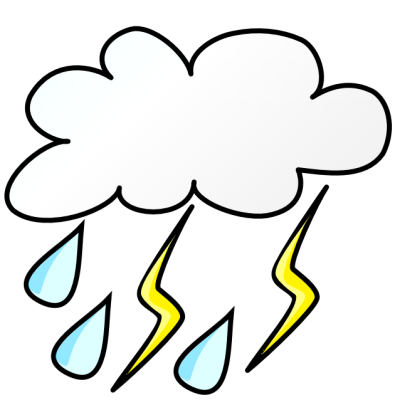
\includegraphics[width=0.2\textwidth]{./imagenes/tormenta.png} 
\caption{Nube de tormenta con rayos y lluvia}
\label{F:tormenta}
\end{figure}

La instrucción para insertar la gráfica es:


\begin{lstlisting}[]
\begin{figure}[H]
\centering
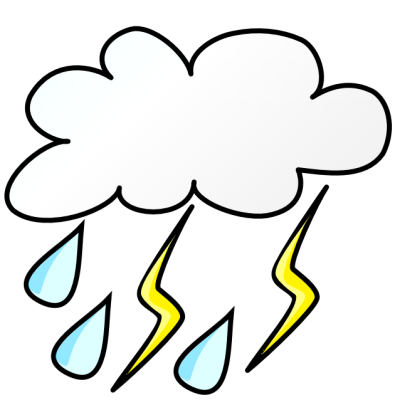
\includegraphics[width=0.2\textwidth]{./imagenes/tormenta.png} 
\caption{Nube de tormenta con rayos y lluvia}
\label{F:tormenta}
\end{figure}
\end{lstlisting}

La descripción es la siguiente:

\begin{itemize}\itemsep0pt \parskip0pt \parsep0pt
\item \verb+\begin{figure}[H]+ en la línea 1 inicia el entorno de la figura y declara que será ubicada inmediatamente luego del texto, con \verb+[H]+.
\item \verb+\centering+ en la línea 2 es una instrucción abreviada para indicar que la figura estará centrada.
\item \verb+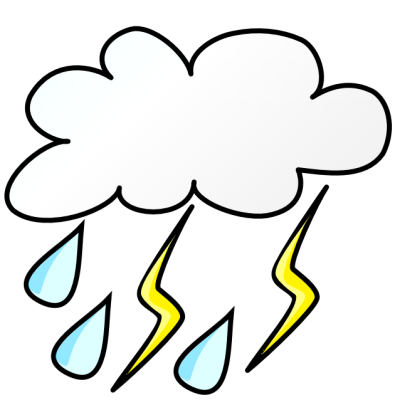
\includegraphics[width=0.2\textwidth]{./imagenes/tormenta.png}+ es la instrucción para insertar el archivo de la imagen, junto con indicaciones adicionales sobre el tamaño (un 20 \% del ancho del texto).
\item \verb+\caption{Nube de tormenta con rayos y lluvia}+ la instrucción  \texttt{caption}\footnote{En inglés, es bastante explícita esta instrucción, y en general puede decirse lo mismo de todos los comandos de \LaTeX, (ver por ejemplo \textsf{footnote}, \textsf{includegraphics}, \textsf{subsection}, etc.)} es el pie de figura con el nombre y la explicación. El número de figura lo inserta \LaTeX~ automáticamente.
\item \verb+\label{F:tormenta}+ es una etiqueta para referencia dentro de otras partes del texto.
\item \verb+\end{figure}+ cierra el entorno de la figura.
\end{itemize}

Como buena práctica, se recomienda nombrar el archivo de la imagen igual que la etiqueta, y con \textit{un nombre representativo}. Los nombres no deben tener espacios ni tildes ni eñes. Por ejemplo: \verb+senal_entrada_sinusoidal.jpg+.

\LaTeX, por defecto, va a ubicar las imágenes arriba o debajo de la página, y no inmediatamente después del texto en el que se escribe dentro del código, excepto que se indique lo contrario con \verb+\begin{figure}[h!]+ o con \verb+\begin{table}[H]+ utilizando el paquete \verb+float+.

Adicionalmente, se puede ubicar varias imágenes dentro de un mismo entorno de figura, como en la Figura \ref{F:subfiguras}. Ahí se muestran cuatro figuras distintas dentro del mismo entorno, donde se puede hacer referencia al transistor en \ref{F:subfig1}, al LED en \ref{F:subfig2}, al fotoconductor en \ref{F:subfig3} y al circuito integrado en \ref{F:subfig4}.

\begin{figure}[h!]
\centering
\subfloat[Transistor (texto que aparece en el índice)][Transistor en encapsulado TO-220]{
	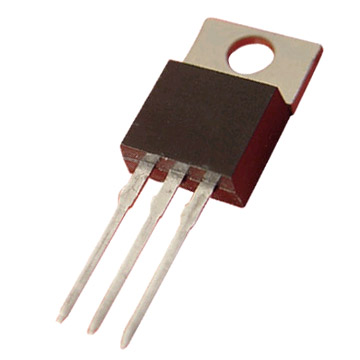
\includegraphics[width=0.2\textwidth]{./imagenes/transistor.jpg}
	\label{F:subfig1}}
\qquad
\subfloat[LED][LED blanco de baja potencia]{
	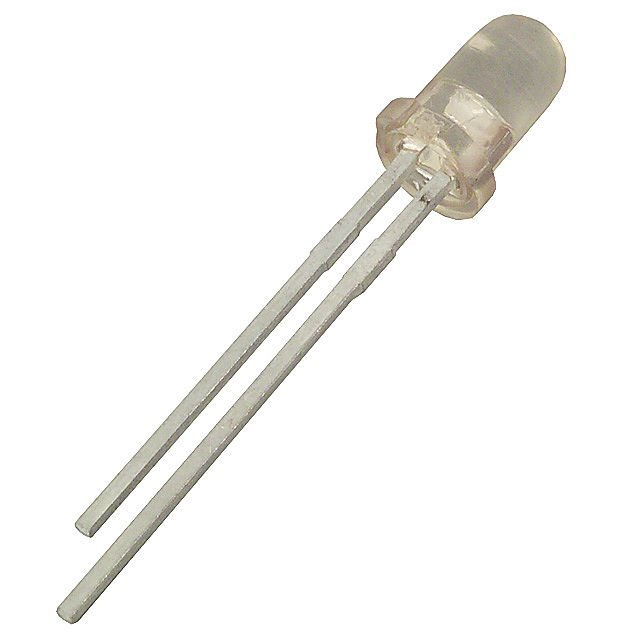
\includegraphics[width=0.2\textwidth]{./imagenes/led.jpg}
	\label{F:subfig2}}
\\
\subfloat[Fotoconductor][Fotoconductor]{
	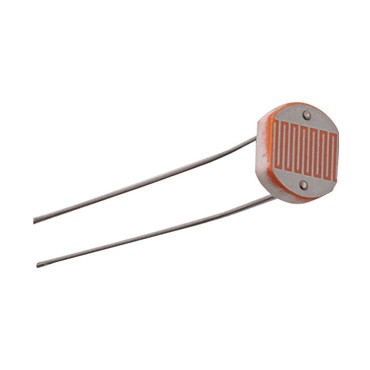
\includegraphics[width=0.2\textwidth]{./imagenes/fotoconductor.jpg}
	\label{F:subfig3}}
\qquad
\subfloat[Circuito integrado][Circuito integrado en encapsulado DIP-8]{
	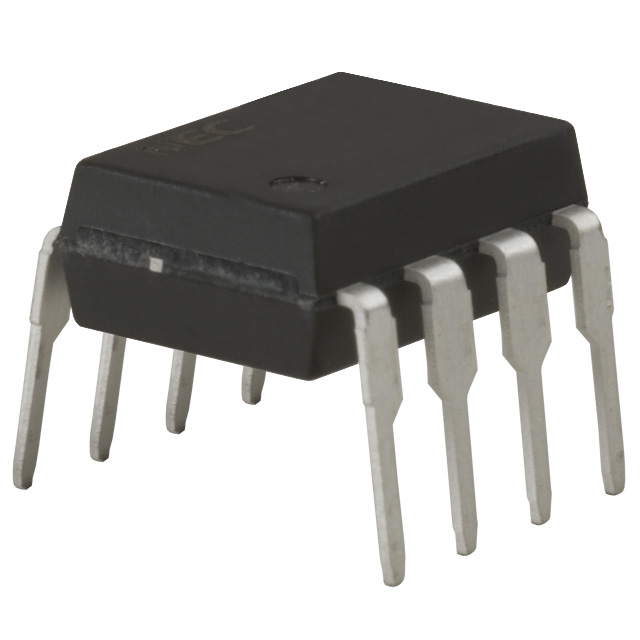
\includegraphics[width=0.2\textwidth]{./imagenes/integrado.jpg}
	\label{F:subfig4}}
\caption{Una figura con varias subfiguras, utilizando el paquete \texttt{subfig}}
\label{F:subfiguras}
\end{figure}

\subsection{Tablas}
%%%%%%%%%%%%%%%%%%%

Para las tablas se debe utilizar el entorno \verb+table+.

Aquí hay dos casos posibles:

\begin{description}

\item [Que la tabla debe construirse en \LaTeX] y en ese caso se debe usar el entorno \verb+tabular+, que a su vez se incluye dentro de \verb+table+.

\item [Que la tabla es en realidad una imagen] si fue generada por otro programa o fue escaneada, etc. Esta imagen entonces se incluye dentro del entorno \verb+table+ para que sea tratada como tal (y se numere como tabla, y se incluya en el índice de tablas, y se hagan las referencias como tablas, etc.).

\end{description}

Como ejemplo sencillo, la Tabla \ref{T:ejemplo} muestra una tabla con líneas verticales, declaradas como \verb+c | c+, que significa \textit{centrado - línea vertical - centrado}, y líneas horizontales, declaradas como \verb+\hline+ después de cada línea salto de línea (\verb+\\+).

\begin{table}
\caption{Comparación de velocidad de UWB con otros estándares alámbricos e inalámbricos}
\label{T:ejemplo}
\begin{center}
\begin{tabular}{ c | c}
\hline
\textbf{Velocidad [Mbits/s]} & \textbf{Estándar} \\ 
\hline
480 & UWB, USB 2.0 \\ 
200 & UWB (4 m) \\
110 & UWB (10 m) \\ 
90 & Fast Ethernet \\ 
54 & 802.11a \\ 
20 & 802.11g \\ 
11 & 802.11b \\ 
10 & Ethernet \\ 
3 & Bluetooth \\ 
0,256 & ZigBee \\ 
\hline
\end{tabular}
\end{center}
\end{table}

La instrucción \verb+\begin{tabular}{ | c | c |}+ genera un cuadro con líneas verticales en ambos lados, como en la Tabla \ref{T:ejemploconlineas}. 

Cuando se tiene un documento de dos o más columnas, es importante notar que una tabla puede ser muy grande y no quepa en una sola columna, por tanto debe especificarse que se acomode a todo lo ancho de la página. Esto es sencillo: basta con escribir \verb+table*+ al inicio y al final cuando se declara el entorno en \verb+\begin{} ... \end{}+.

\begin{table*}
\caption[Título en el índice]{Título que aparece en el pie de figura o encabezado de la tabla. Puede ser bastante amplio y explicar con más detalle. Debido a que el título que aparece en el índice es corto, no hay problema de que se exceda el espacio apropiado ahí.}
\label{T:ejemploconlineas}
\begin{center}
\begin{tabular}{| c | c |}
\hline
\textbf{Velocidad [Mbits/s]} & \textbf{Estándar} \\ 
\hline
480 & UWB, USB 2.0 \\ 
200 & UWB (4 m), 1394a (4,5 m) \\
110 & UWB (10 m) \\ 
90 & Fast Ethernet \\ 
54 & 802.11a \\ 
20 & 802.11g \\ 
11 & 802.11b \\ 
10 & Ethernet \\ 
3 & Bluetooth \\ 
0,256 & ZigBee \\ 
\hline
\end{tabular}
\end{center}
\end{table*}

Del mismo modo que en las figuras, \LaTeX~ por defecto colocará la tabla en la parte superior de la siguiente página, excepto que se indique lo contrario (con \verb+\begin{table}[h!]+)\footnote{Para mejor manejo de la posición de figuras, tablas y otros, utilizar el paquete \textsf{float}}.

\begin{table}
\caption{Otra tabla utilizando el paquete \texttt{booktabs}}
\label{T:otratabla}
\centering
\begin{tabular}{c l r r}
\toprule
\multicolumn{2}{c}{Producto} \\
\cmidrule(r){1-2}
Cantidad & Descripción & Precio unitario & Precio total  \\
\midrule
3  & Transistores 	& 250	& 750	\\
4  & Osciladores   	& 500   & 2000 \\
3  & Amp Ops     	& 600   & 1800	\\
10 & Resistores  	& 25    & 250	\\
10 & Capacitores	& 50 	& 500	\\
\midrule 
\multicolumn{3}{r}{TOTAL} & \textbf{5300} \\
\bottomrule
\end{tabular}
\end{table}

%%%%%%%%%%%%%%%%%%%%%%%%%%%%%
\section{Herramientas útiles}
%%%%%%%%%%%%%%%%%%%%%%%%%%%%%

%----------------------------------
\subsection{Referencias a figuras, tablas, ecuaciones, secciones y otros}

Es fundamental a lo largo del texto hacer referencias a figuras, tablas, ecuaciones, secciones y otros. Todos estos elementos tienen una etiqueta \verb+\label{}+ asociada a cada uno. 

La instrucción para hacer la referencia a esta etiqueta es \verb+\ref{}+.

Así entonces, se puede hacer referencia a las ecuaciones (\ref{E:desigualdad}), (\ref{E:anchodebanda}) y (\ref{E:fraccional}), a la Figura \ref{F:tormenta} y a la Tabla \ref{T:ejemplo} desde cualquier parte del texto, sin importar la numeración, que será asignada automáticamente por \LaTeX.

Es buena práctica nombrar las ecuaciones como \verb+\label{E:ecuacion}+, las tablas como \verb+\label{T:tabla}+, las figuras como \verb+\label{F:figura}+, y así sucesivamente, es decir, con una E, T, F o S antepuestas para identificar de qué se trata en cada caso, y con un nombre representativo. 

No es bueno hacer referencias relativas como ``la siguiente figura'' o ``la tabla anterior'' porque en realidad no se sabe la ubicación final dentro del texto. Hay que notar que tanto las tablas como las figuras, a menos de que se especifique lo contrario\footnote{Como se ha explicado, una forma de cambiar esto es colocando [h!] o [H] (de \emph{here}) junto al inicio del entorno.}, se colocarán al principio o al final de la página, en donde el programa lo considere mejor por motivo de espacio. Es mejor una referencia absoluta tal como figura \ref{F:tormenta} o ecuación (\ref{E:fraccional}). 

En editores de escritorio, algunas veces es necesario compilar dos o tres veces para que se carguen correctamente los números de referencia.

\subsection{Citas bibliográficas}
%%%%%%%%%%%%%%%%%%%%%%%%%%%%%%%%%

Los trabajos académicos requieren de referencias a las fuentes de información, invariablemente. Es necesario entonces considerar cómo crear una bibliografía y cómo referirse a las fuentes dentro del texto. 

Se puede hacer una bibliografía ``a mano'', en el que se le da la edición necesaria a cada entrada\footnote{En el código fuente de este documento hay un ejemplo de bibliografía tipo ``plain''.}. Sin embargo, BibTeX es una mejor alternativa, que permite administrar y modificar fácilmente una gran cantidad de entradas, además de que hace posible la reutilización de las referencias, en otros documentos.

\subsubsection{BibTeX}

\href{http://www.bibtex.org/}{BibTeX} es un programa de manejo de referencias. En este documento se utiliza de la siguiente forma:

\begin{itemize}
\item En un archivo llamado \texttt{bibliografia.bib} se introducen todas las referencias utilizadas, con el formato especial para ello. Ejemplo:
\begin{verbatim}
@BOOK {Valiente2001,
    author    = "Valiente Feruglio, G.",
    title     = "Composición de Textos Científicos con LaTeX",
    publisher = "Alfaomega",
    year      = "2001",
    address   = "México D.F.",
    edition   = "primera"
}
\end{verbatim}
Una buena herramienta para editar estas entradas se encuentra en \url{http://truben.no/latex/bibtex/}, sin embargo, considerar los sistemas de manejo bibliográfico de la siguiente sección.

\item Dentro del texto se hace referencia a las fuentes. La instrucción para hacer una cita es \verb+\cite{+\textit{clave}\verb+}+, dentro del cual se coloca la etiqueta, clave o \textit{key} asignada a la bibliografía (el primer espacio en la entrada de BibTeX de ejemplo), usualmente el apellido del primer autor y el año de publicación, por ejemplo: \verb+\cite{Valiente2001}+, que resulta en \cite{Valiente2001}.

\item Finalmente, al final del trabajo, se colocan las instrucciones 
\begin{verbatim}
\bibliographystyle{estilo}
\bibliography{nombrearchivo.bib}
\end{verbatim}
donde \texttt{estilo} es uno de los varios formatos posibles para las citas y las referencias (ver una lista en \url{https://www.sharelatex.com/learn/Bibtex_bibliography_styles}), y la segunda instrucción se encarga de colocar el título, y todas las entradas \textbf{que han sido citadas}, en el orden y el formato necesarios. Ahí es donde la ventaja de BibTeX se hace más evidente. 

\item En programas de edición de escritorio (Texmaker,\ldots) es necesario compilar varias veces y en una secuencia específica para que se genere la bibliografía. Esta secuencia es: \texttt{latex} \textgreater~ \texttt{bibtex} \textgreater~ \texttt{latex} \textgreater~ \texttt{latex}. En las plataformas de edición en línea (Overleaf,\ldots) esto se hace automáticamente.
\end{itemize}

\subsubsection{Sistemas de manejo bibliográfico}

En trabajos de investigación es necesario recurrir a muchas referencias (en tesis y otros, fácilmente más de 50) y el manejo de estas se puede tornar engorroso. Actualmente, varias plataformas ofrecen un manejo automatizado y muy conveniente de referencias. A continuación se presentan algunas opciones.

\begin{multicols}{2}
\begin{description}
\item[Mendeley] \url{http://www.mendeley.com/}
\item[Readcube] \url{http://www.readcube.com/}
\item[Docear] \url{http://www.docear.org/}
\item[Citavi] \url{http://www.citavi.com/}
\item[EndNote] \url{http://endnote.com/}
\item[JabRef] \url{http://jabref.sourceforge.net/}
\end{description}
\end{multicols}

\subsection{Formato}
%%%%%%%%%%%%%%%%%%%%

%---------------------------------------
\subsubsection{Cambiar el tipo de letra}

La tipografía de \LaTeX~ por defecto es la \href{https://en.wikipedia.org/wiki/Computer_Modern}{Computer Modern}. Es fácil de identificar y ampliamente utilizada (por la popularidad de \LaTeX) en muchas publicaciones científicas.

Esta plantilla de Proyecto Eléctrico utiliza la tipografía \href{http://www.linuxlibertine.org/}{Libertine}. 

Es útil, sin embargo, cambiar de tipografía en todo el documento o en algunas secciones\footnote{¡Cuidado! Demasiada libertad para cambiar el formato del documento puede derivar en malas decisiones de diseño gráfico. Ejemplo usual: utilizar Comic Sans (no disponible aquí).}.

Una referencia de la mayoría de tipografías disponibles para \LaTeX~ se encuentra en \url{http://www.tug.dk/FontCatalogue/}. Por ejemplo, la siguiente instrucción en el preámbulo convierte todo el texto a DejaVu Sans.

\begin{verbatim}
\usepackage{DejaVuSans}
\renewcommand*\familydefault{\sfdefault} 
\usepackage[T1]{fontenc}
\end{verbatim}

La instrucción \verb+{\fontfamily{qag}\selectfont ...texto...}+ genera {\fontfamily{qag}\selectfont un texto en otra tipografía. Para restringir la selección, el texto debe estar rodeado por llaves}. El código \texttt{qag} representa el tipo de letra. Una lista de tipos de letras y sus códigos, junto con más opciones se puede encontrar \href{https://www.sharelatex.com/learn/Font_typefaces}{aquí} y \href{http://tex.stackexchange.com/questions/25249/how-do-i-use-a-particular-font-for-a-small-section-of-text-in-my-document}{aquí}.

%-----------------------
\subsubsection{Unidades}

Las unidades deben escribirse separadas de la magnitud. Cuando se hace en una ecuación se presenta el problema que muestra la ecuación (\ref{E:sinunidades}). Para resolver este problema hay que incluir algún paquete que permita introducir unidades correctamente. En este documento se eligió \verb+siunitx+. La ecuación (\ref{E:conunidades}) muestra el uso corregido de las unidades en las ecuaciones. Del mismo modo, se puede poner de ejemplo: $C_s = \SI{0.1}{\micro\farad}$, $T_c = \SI{27}{\degreeCelsius}$. 

\begin{equation}\label{E:sinunidades}
{V}_{i}\ge 1,3 mV
\end{equation}

\begin{equation}\label{E:conunidades}
{V}_{i} \ge 1,3~\si{\milli\volt}
\end{equation}

O también el siguiente ejemplo:

\begin{equation}\label{E:unidades}
V = I_L \times R_L = \left( 0,25~\si{\milli\ampere} \right) \times \left( \SI{4}{\kilo\ohm} \right) = 1~\si{\volt} 
\end{equation}

%--------------------------------------------
\subsubsection{Otras herramientas de formato}

\begin{enumerate}
\item Las notas de pie\footnote{Que se insertan escribiendo la instrucción inmediatamente después del texto a comentar, como en este caso.}, utilizando la instrucción \verb+\footnote{}+.
\item Las comillas, que colocan con estos símbolos ``especiales'' y no las comillas del teclado. 
\item La palabra \LaTeX~ se escribe con el comando \verb+\LaTeX+. Debe escribirse el símbolo \verb+~+ después de la instrucción para que genere un espacio adecuado entre palabras, de otro modo \LaTeX queda pegado.
\item Las \textbf{negritas} se escriben con el comando \verb+\textbf{}+ (de \textit{\textbf{b}old \textbf{f}ace})
\item Las \textit{cursivas} se escriben con el comando \verb+\textit{}+ (de \textit{\textbf{it}alics})
\item Las \textsc{versales} se escriben con el comando \verb+\textsc{}+ (de \textit{\textbf{s}mall \textbf{c}aps})
\item Las \texttt{monoespacio} se escriben con el comando \verb+\texttt{}+ (de \textit{\textbf{t}ele\textbf{t}ype})
\item El comando \verb+\emph{}+ se utiliza para \emph{resaltar} un texto, muy similar a \verb+\textit{}+, con la diferencia que \textit{el resaltado depende del \emph{contexto} del párrafo}.
\item Hay varios tamaños de guiones: -, -- (con \verb+--+) y --- (con \verb+---+).
\item Se puede especificar la fecha de hoy, \today, utilizando el comando \verb+\today+.
\item El paquete \verb+hyperref+ permite la inclusión de hipervínculos, tanto a lugares externos del documento como internos (observe las referencias a tablas, figuras o ecuaciones o las citas bibliográficas). También incorpora los   marcadores que se muestran en los lectores de pdf y que se utilizan para navegación del documento. Por ejemplo, se puede hacer referencia a la Sección \ref{S:Figuras} donde se explica la inclusión de figuras (y hacer clic al hipervínculo y seguirlo).
\item Las listas numeradas (como esta) se hacen con el entorno \verb+\begin{enumerate}+, las listas con viñetas utilizando \verb+\begin{itemize}+.
\item Se pueden crear comandos especiales para insertar textos o símbolos definidos por el usuario. La instrucción es \verb+\newcommand{\comando}{Texto a introducir}+.
\item Por ejemplo, si no se quiere escribir cada vez ``Escuela de Ingeniería Eléctrica'' y además se le quiere dar un formato especial, entonces se puede indicar en el preámbulo 

\verb+\newcommand{\EIEx}{\textsc{Escuela \Lightning~ Ingeniería Eléctrica}}+ 

y así se crea el comando \verb+\EIEx+ que genera: \EIEx.
\item[--] Se puede utilizar un guión (o cualquier símbolo) en lugar de la numeración o las viñetas en una lista, con la instrucción \verb+[-]+ al lado de \verb+\item+.
\item[\Biohazard] Ejemplo de símbolo como viñeta\footnote{Las instrucciones \texttt{Lightning} y \texttt{Biohazard} son parte del paquete de símbolos especiales \texttt{marvosym}.}.
\end{enumerate}

\subsection{Figuras con PGF/Ti\textit{k}Z}
%%%%%%%%%%%%%%%%%%%%%%%%%%%%%%%%%%%%%%%%%%

PGF/Ti\textit{k}Z es un conjunto de lenguajes para producir gráficos vectoriales a partir de una descripción geométrica y algebraica\footnote{Tomado de su descripción en Wikipedia.}. Tiene grandes capacidades y una documentación exhaustiva.

La Figura \ref{F:tikz} es un ejemplo relativamente sencillo de las capacidades de Ti\textit{k}Z.

\begin{figure}[H]
\centering
	\begin{tikzpicture}
	  \draw[fill=yellow] (0,0) -- (60:.75cm) arc (60:180:.75cm);
	  \draw(120:0.4cm) node {$\alpha$};
	  \draw[fill=green!30] (0,0) -- (right:.75cm) arc (0:60:.75cm);
	  \draw(30:0.5cm) node {$\beta$};
	  \begin{scope}[shift={(60:2cm)}]
	    \draw[fill=green!30] (0,0) -- (180:.75cm) arc (180:240:.75cm);
	    \draw (30:-0.5cm) node {$\gamma$};
	    \draw[fill=yellow] (0,0) -- (240:.75cm) arc (240:360:.75cm);
	    \draw (-60:0.4cm) node {$\delta$};
	  \end{scope}
	  \begin{scope}[thick]
	    \draw  (60:-1cm) node[fill=white] {$E$} -- (60:3cm) node[fill=white] {$F$};
	    \draw[red]                   (-2,0) node[left] {$A$} -- (3,0) node[right]{$B$};
	    \draw[blue,shift={(60:2cm)}] (-3,0) node[left] {$C$} -- (2,0) node[right]{$D$};
	    \draw[shift={(60:1cm)},xshift=4cm]
	    node [right,text width=6cm,rounded corners,fill=red!20,inner sep=1ex]
	    {
	      Cuando asumimos que $\color{red}AB$ y $\color{blue}CD$ son paralelos, es decir, ${\color{red}AB} \mathbin{\|} \color{blue}CD$, entonces $\alpha = \delta$ y $\beta = \gamma$.
	    };
	  \end{scope}
	\end{tikzpicture}
\caption[Ejemplo de uso de PGF/Ti\textit{k}Z]{Ejemplo de uso de PGF/Ti\textit{k}Z, pero solo una muestra de sus capacidades.}
\label{F:tikz}
\end{figure}

Una buena cantidad de ejemplos están disponibles en \url{http://www.texample.net/tikz/} y la documentación (incluyendo un manual de uso de más de 700 páginas) está en \url{https://www.ctan.org/pkg/pgf?lang=en}.

%---------------------------------------
\subsection{Gráfico de datos y funciones con \texttt{pgfplots}}

%---------------------------------------
\subsection{Circuitos con Circuitikz}

El paquete \texttt{circuitikz} permite la creación de circuitos eléctricos y electrónicos. La Figura \ref{F:ampop} es un ejemplo.

\begin{figure}
  	\centering
		 \begin{circuitikz}[american]
		  \draw
		  % El amplificador operacional
		  (0,0) node[op amp] (opamp) {} node[] {{\tiny Amp Op}}
		  
		  % Las entradas
		  (opamp.-) node[circ] {} to[R, l_=$R_1$] ++(-2,0) node[ocirc] {} node[left] {$V_{s}$}
		  (opamp.+) -- ++(0,-0.5) node[ground] {} 
		  
		  % El lazo de realimentación
		  (opamp.-) -- ++(0,1)  to[R, l=$R_2$] ++(2,0) -| (opamp.out) {}
		  
		  % La salida
		  (opamp.out) -- ++(0.5,0) node[circ] {} to[R, l=$R_L$] ++(0,-2) to [short, i_=$I_o$] ++(0,0) node[ground] {}
		  (opamp.out) -- ++(1,0) node[ocirc] {} node[right]{$V_o$}
		  
		  ;
		\end{circuitikz}
    \caption[Amplificador inversor]{Amplificador inversor con un amplificador operacional cuya relación entrada--salida está dada por $V_o = -\frac{R_2}{R_1} V_s$.}
    \label{F:ampop}
\end{figure}

\begin{figure}
\centering
\begin{circuitikz}
\draw
	(0,0)
    	to [V, l=50~\si{\volt}] (0,2) to (0,3)
        to [R, l=$20~\si{\kilo\ohm}$] (5,3) to (5,2)
        to [vR, l=$R$] (5,0)
        to (0,0)
  	(0,2)
    	to [R, l_=$5~\si{\kilo\ohm}$] (5,2)     
;
\end{circuitikz}
\caption{Circuito básico.}
\label{F:circuitobasico}
\end{figure}

\begin{figure}
\centering
\begin{circuitikz}
\draw
	(0,0) node[ground]{}
    	to [V, l=(``Arenal'') $V_{1}$] (0,3)
        to [short] (0.5,3) node[circ]{}
   	(5.5,3)
        to [short] (5.5,4)
        to [R, l=$R_{1}$, i<=$I_{1}$] (3,4)
        to [cV, l=$v_{1}$] (0.5,4)
        to [short] (0.5,3)   
   	(6,3)
    	to [short] (5.5,3)
        to [short] (5.5,2)
        to [R, l=$R_{3}$, i<=$I_{2}$] (3,2)
        to [cV, l=$v_{3}$] (0.5,2)
        to [short] (0.5,3)
	(6,3) node[circ]{}
    	to [generic, i_=$I_{L}$, v^=$v_{L}$] (6,0) node[ground]{}
   	(6,3)
    	to [R, l=$R_{2}$, i<=$I_{3}$] (8.5,3)
        to [cV, l=$v_{2}$] (11,3)
    (11,0) node[ground]{}
        to [V, l_=$V_{2}$ (``Miravalles'')] (11,3)
;
\end{circuitikz}
\caption[Circuito de transmisión de potencia]{Circuito de transmisión de potencia por varias líneas conductoras desde centros de generación y con sistemas de ajuste de la corriente.}
\label{F:transmisionpotencia}
\end{figure}

\begin{figure}
\centering
\begin{circuitikz}
\draw 
(0,0)	to [battery, l_=$V_i$] (0,3)
		to [R, l_=$R_1$] (2.5,3)
        to [cV, l_=$A v_x$] (5,3)
        to [short] (6,3)
        to [vR, l_=$R_T$, i=$i_{R_T}$] (6,0) node[ground]{}
        to [short] (0,0)
(6,3)	to [short] (7,3)
(6,0)	to [short] (7,0)

;
\draw (2.5,3) to [open, v=$v_x$] (2.5,0);
\draw (2.5,3) node[circ]{};
\draw (2.5,0) node[circ]{};

\draw[dashed] (-0.8,-0.8) rectangle (4.8,3.8);
\draw (-0.8,-0.8) node [above right]{Fuente de corriente};

\draw (7,-0.5) rectangle (9,3.5);
\draw (8,1.5) node [align=center]{Circuito \\ de acople};

\draw 
(9,3)	to [short] (10,3)
		to [R, l_=$R_2$] (12,3)
		to [generic, l_=$Y$, v^=$v_Y$] (14,3)
(9,0)   to [short] (14,0) node[ground]{}
		to [cV, l=$A v_z$] (14,3)
(14,0)	to [short] (15.3,0)
		to [open, v>=$v_o$] (15.3,3)
		to [short] (14,3)
;
\draw (12,3)	to [open, v=$v_z$] (12,0);
\draw (12,3) node[circ]{};
\draw (12,0) node[circ]{};

\draw[dashed] (9.8,-0.8) rectangle (14.8,3.8);
\draw (9.8,-0.8) node [above right]{Amplificador};

\draw (15.3,3) node[circ]{} node[right]{$a$};
\draw (15.3,0) node[circ]{} node[right]{$b$};
\end{circuitikz}
\caption[Circuito de acondicionamiento y amplificación]{Circuito de acondicionamiento y amplificación de la señal de un sensor resistivo $R_T$, dependiente de la temperatura.}
\label{F:acondicionamiento}
\end{figure}

\begin{figure}
\centering
\begin{circuitikz}

% PNP Q1
\draw
	(0,4) 	node[pnp,rotate=90](Q1){} node[above]{$Q_1$}
;
% NPN Q2
\draw
	(0,1.5) 	node[npn,rotate=180,yscale=-1](Q2){} node[left]{$Q_2$}
;
% Op Amp
\draw
	(3,1.5) 	node[op amp,rotate=180,yscale=-1](CMP){} node[]{AMP}
;
% Resistores
\draw
	(6,4) node[circ]{} 
    	to [R, l=$R_1$] (6,2) 
    	to [R, l=$R_2$] (6,0) node[ground]{}
;
% Conectores
\draw
	(-1.5,4) 	node[ocirc]{} node[above]{$V_{IN}$} 
    		to [short] (Q1.emitter)
  	(Q1.base) to [short] (Q2.collector)
    (Q2.emitter) to [short] (0,0) node[ground]{}
    (CMP.out) to [short] (Q2.base)
    (Q1.collector) to [short] (7,4) node[ocirc]{} node[above]{$V_{OUT}$}
    (CMP.-) to [short] (6,2) node[circ]{}
    (4.5,0) node[ground]{} to [battery,l_=$V_{R}$] (4.5,1) to [short] (CMP.+) 
;
\end{circuitikz}
\caption{Regulador lineal de tensión con lazo de control.}
\label{F:reguladorlineal}
\end{figure}

\begin{figure}
\centering
\begin{circuitikz} 
\draw
	(0,0) node[op amp,yscale=-1] (opamp) {}
    (0,0) node[](){CMP}
;

\draw 
	(-4.5,2) node[rground, yscale=-1](){} 
    to [I, l_=$I$] (-4.5,1)
    to [short,-*] (-4.5,0.5)
    to [short] (-4.5,-1.8) 
;

\draw 
	(-3,2) node[rground, yscale=-1](){} 
    to [I, l_=$I$] (-3,1)
    to [short,-*] (-3,-0.5) 
    to [R, l_=$R_1$] (-3,-2.5)
    to [R, l_=$R_2$] (-3,-4.5) node[ground](){}
;

\draw 
	(-3,-2.5) to [short,*-] (-2,-2.5)
    to [cspst,] (-2,-4.5) 
    to [short] (-3,-4.5)
    (-1.8,-3.8) node[right](){SW}
;

\draw 
	(-4.5,-2.5) node[pnp](pnp){}
	(pnp.base) node[anchor=east] {\tiny{B}}
    to [short] (-5.3,-4.5) to [short,-*] (-4.5,-4.5)
    (pnp.emitter) node[anchor=east]{\tiny{E}} 
    (pnp.collector) node[anchor=east] {\tiny{C}}
    to [short] (-4.5,-4.5) to [short,-*] (-3,-4.5)
    (-4.5,-2.5) node[anchor=west] {$Q_T$}
;

\draw (opamp.-) to [short] (-3,-0.5) node[anchor=east]{$V^-$};
\draw (opamp.+) to [short] (-4.5,0.5) node[anchor=east]{$V^+$};
\draw (opamp.out) to [short] (1.5,0);
\draw[dashed] (1.5,0) -- (1.5,-3.4) -- (-1.7,-3.4);

\draw (4,0)  node[ocirc]{} node[anchor=south]{\={S}} to [full diode] (1.5,0) node[circ]{} node[anchor=south]{$V_{\mathrm{CMP}}$};

\end{circuitikz}
\caption{Circuito para protección térmica con lazo de histéresis.}
\label{F:protecciontermica}
\end{figure}

\subsection{Inserción de código fuente}
%%%%%%%%%%%%%%%%%%%%%%%%%%%%%%%%%%%%%%%

En ocasiones es necesario introducir secciones de código fuente de programación dentro de reportes. La inserción es especial, pues el compilador no debe confundir las instrucciones dentro del código con instrucciones de \LaTeX. Además, se prefiere un formato específico con resaltado de sintaxis para mejorar la legibilidad (como en los editores de código o en los IDE). Un paquete que provee soluciones para este requisito es \texttt{listings}.

Para el código fuente hecho en Matlab es posible utilizar el paquete \texttt{mcode} (adjunto como archivo a la carpeta que contiene el proyecto) que asigna a \texttt{listings} el formato apropiado, como se ve en el siguiente código:

\lstinputlisting[inputencoding=latin1]{codigo/codigoejemplo.m}

%%%%%%%%%%%%%%%%%%%%%%%%%%%%%%%%%
\section{Referencias para \LaTeX}
%%%%%%%%%%%%%%%%%%%%%%%%%%%%%%%%%

La comunidad de usuarios de \LaTeX~ es grande y colaborativa. Hay multitud de recursos en línea para aprender buenas prácticas y ``trucos'' para mejorar los documentos. Algunas de las mejores referencias son:

\begin{description}
\item[Wikibook] \url{https://en.wikibooks.org/wiki/LaTeX}
\item[Cookbook] \url{http://latex-cookbook.net/}
\item[TeXample] \url{http://texample.net/}
\item[HowtoTeX] \url{http://www.howtotex.com/}
\item[Font Catalogue] \url{http://www.tug.dk/FontCatalogue/}
\end{description}

\subsection{¿Dónde editar \LaTeX?}\label{S:programas}
%%%%%%%%%%%%%%%%%%%%%%%%%%%%%%%%%%%%%%%%%%%

\paragraph{Editores de texto ``de escritorio''}

Existen varios programas para la edición y compilación de archivos de \LaTeX. Se ha escogido Texmaker debido a que es multiplataforma (Mac, Linux, Windows) y cuenta con otras características como resaltado de sintaxis, autocompletar, corrección ortográfica, asistente para la creación de documentos, accesos rápidos a símbolos, comandos y entornos, entre otros. Se puede, claro está, editar el documento con cualquier editor y compilar, siempre y cuando se tengan los paquetes necesarios\footnote{Esta es una ventaja de ser un código estándar abierto.}.

En Windows, junto con Texmaker debe instalarse MiKTeX, que es un conjunto de paquetes, fuentes y demás necesarios para compilar el archivo.

Ambos están disponibles para descarga gratuita desde \url{http://miktex.org/} y \url{http://www.xm1math.net/texmaker/}.

Una base de datos extensiva de los paquetes de \LaTeX~ está en \url{http://www.ctan.org/}. Es especialmente útil para encontrar la documentación de los paquetes. Desde esta página se pueden descargar los paquetes, pero la mejor forma de revisar los paquetes disponibles e instalarlos fácilmente es a través del \emph{MiKTeX Package Manager}, disponible después de instalar el MiKTeX.

\paragraph{Plataformas en línea de edición para \LaTeX}

Una alternativa muy popular de años muy recientes es la edición en línea. Entre las ventajas se encuentran: almacenamiento en línea, edición colaborativa, herramientas web (bibliografías y otros), compilación simultánea, más la mayoría de las otras ventajas de los editores ``de escritorio'' como autocompletar, símbolos, etc.

Los editores más populares son:

\begin{description}
\item[Overleaf] \url{https://www.overleaf.com/}
\item[ShareLaTeX] \url{https://www.sharelatex.com/}
\item[Papeeria] \url{https://papeeria.com/}
\end{description}